% !TEX root = ../main.tex
% !TEX root = ../main.tex

\ours~is a visual analytics system designed to support historians in their practice of mention gathering and analysis.
The system is unique within a large literature on text analytics because it is designed to help analyze query mentions in context, which constitute the system's central ``unit of analysis'' (this terminology comes from Chuang et al.\ \cite{chuangheer}). 
By contrast, prior text analytics tools focus on the investigation of other units of analysis like topics \cite{tiara}, events \cite{eventriver}, or thematic hierarchies \cite{overview} (see Section \ref{s:related_comparison}).

\ours's unique focus on query mentions in context reflects our study into the needs and practices of historical researchers, who helped refine early iterative prototypes \cite{GouldClayton}.
Because such historians need to quickly and comprehensively review occurrences of a query word in a large corpus, \ours~uses text simplification techniques (Section \ref{s:simplification}) to create a skimmable summary of a query across an archive. 
Such text simplification techniques and skimmable summaries are unique within the large literature on text analytics, and thus constitute the chief technical contribution of our work.
We hypothesize that this query-focused summarization, along with \ours's~linked views, in-text highlighting, and history tracking features, can help experts quickly, comprehensively, and transparently gather and analyze \mentions, the comprehensive set of all mentions of a query in a news archive.

\subsection{High-level system description}\label{s:highlevell}

The \ours~web interface presents results from a Boolean search \cite[Chapter 1]{irbook}, which returns the unranked set of documents containing one or more mentions~of a unigram query term \Q~in an archive \archive. 
(This notation and terminology is defined in Section \ref{s:needs_formal_problem}; Section \ref{s:limits_and_future} discusses possible extensions to exact string matching.)
When a user enters $Q$ into the search bar at the top of the interface (Figure \ref{f:system_cc}A), \ours~identifies all documents containing $Q$ and presents the documents using three linked views \cite{BujaLinking}. 
First, \ours~includes a \textbf{Time Series View}, showing a graphical overview of the count of documents mentioning the query by year (Figure \ref{f:system_cc}D). 
Second, \ours~includes a \textbf{Document Feed} view, presenting all query mentions from across all documents in a single scrollable window (Figure \ref{f:system_cc}H).
Finally, \ours~includes a \textbf{Document Viewer}, which shows the full text of a single document from the corpus, with individual query mentions from the document highlighted in context (Figure \ref{f:system_cc}I).
\ours~also includes a \textbf{filtering system} to help users narrow the set of query mentions shown in the interface (Figure \ref{f:system_cc}B, C and F), and a \textbf{history tracking system} to automatically monitor and display reading history during comprehensive search (Figure \ref{f:system_cc}G).
All features in the interface also follow a coordinated \textbf{color coding} scheme.
For instance, the user's query word is always displayed using the purple query color {
\includegraphics[scale=0.06]{figures/CCPurple.pdf}} in the Document Feed and Document Viewer, and the Time Series View also uses a {purple} line to represent query frequency (Figure \ref{f:system_cc}D).
We consider the color-coded bolding of query terms to be one form of \textbf{automatic in-text highlighting} \cite{Handler2016VisualizingTM} throughout the \ours~interface.
Automatic in-text highlighting draws user attention to some word, phrase, or passage in text by automatically setting the text's foreground color, background color or decoration (e.g., bolding).
The Appendix describes our process for selecting a colorblind safe and print-friendly palette. 
It also provides additional engineering details about our implementation of \ours.


\subsection{Overview first: a Time Series View for temporal context (\roverview)}\label{s:system_ts}

Because change across time is central to historical research (\roverview),~\ours~presents a navigable Time Series View (Figure \ref{f:system_cc}D) showing query frequency by year across a corpus.
The component's x-axis represents time (binned by year), and its y-axis represents the annual count of all documents containing the query \Q~published during a given year.
If a user also enters a subquery (Section \ref{s:dont_rank_filter}), \ours's Time Series View also shows the annual count of documents mentioning both the query and subquery.
In Figure \ref{f:system_cc}D, \ours~displays one line showing the count of documents mentioning the query term in the purple query color, and another line showing the count of documents mentioning the subquery term (as well as the query term) in the green subquery color 
\includegraphics[scale=0.06]{figures/CCGreen.pdf}.
\ours's time series plot also shows a single rug point (small vertical line) for each document mentioning the query, just beneath the temporal x-axis (Figure \ref{f:system_cc}E).
Such rug points allow the user to easily preview and navigate to individual news stories; we describe these possible interactions in detail in the Appendix.

\subsection{A Document Feed for comprehensive search (\rcomprehensive)}\label{s:feed_and_viewer}

During needfinding, we found that experts often emphasized the importance of gathering comprehensive evidence (Section \ref{s:needs_comprehensive}), and also often search for specific query terms in news archives (Section \ref{s:intro}).
We thus designed \ours's {Document Feed} to help such users easily gather and analyze the comprehensive set of every single mention of a query term in a collection of news stories (\rcomprehensive).
We assume the user is working with a small corpus (or small set of documents from a larger corpus), where such comprehensive review is possible. 
This assumption is appropriate for our use case; 
for instance, Black reviews roughly 500 documents to analyze the racial history of ``watermelon,'' \cite{watermelon} and MacNamara reviews 605 documents to analyze ``race suicide'' \cite{racesuicide}.

After a user issues a query $Q$, \ours~populates the Document Feed to show a comprehensive, skimmable, summary which includes every single \specificmention~across the corpus (Figure \ref{f:system_cc}J). 
To create the summary, \ours~selects each sentence containing some \specificmention, and then automatically simplifies the sentence (without removing query words) so that historians can quickly read over the mention $i$ in context.
We use the notation \simplifiedsentence~to refer to a specific query mention \specificmention~shown within the context of a sentence $s$ that is simplified to $s^\prime$ for display in the Document Feed.
Section \ref{s:text_simplification_overview} provides details on how \ours~shortens sentences to create~\simplifiedsentence. To the best our knowledge, such text simplification is new to the literature on text analytics.
In presenting each~\simplifiedsentence, \ours~bolds and highlights the query word using the purple query color so that each \simplifiedsentence~is shown in a visually consistent format designed for skimming (Figure \ref{f:compressioncartoon}). 

Note that by default, \ours~displays a single~\simplifiedsentence~from each document beneath the document's headline (The Appendix describes how the sentence is chosen).
To see each \specificmention~from a document within a simplified sentence, the user can click an ``expand'' button (Figure \ref{f:field_study_loop}). 
The user can also click a star to bookmark a document in the red bookmark color 
\includegraphics[scale=0.06]{figures/CCRed.pdf}.



\begin{figure}[ht]
\centering
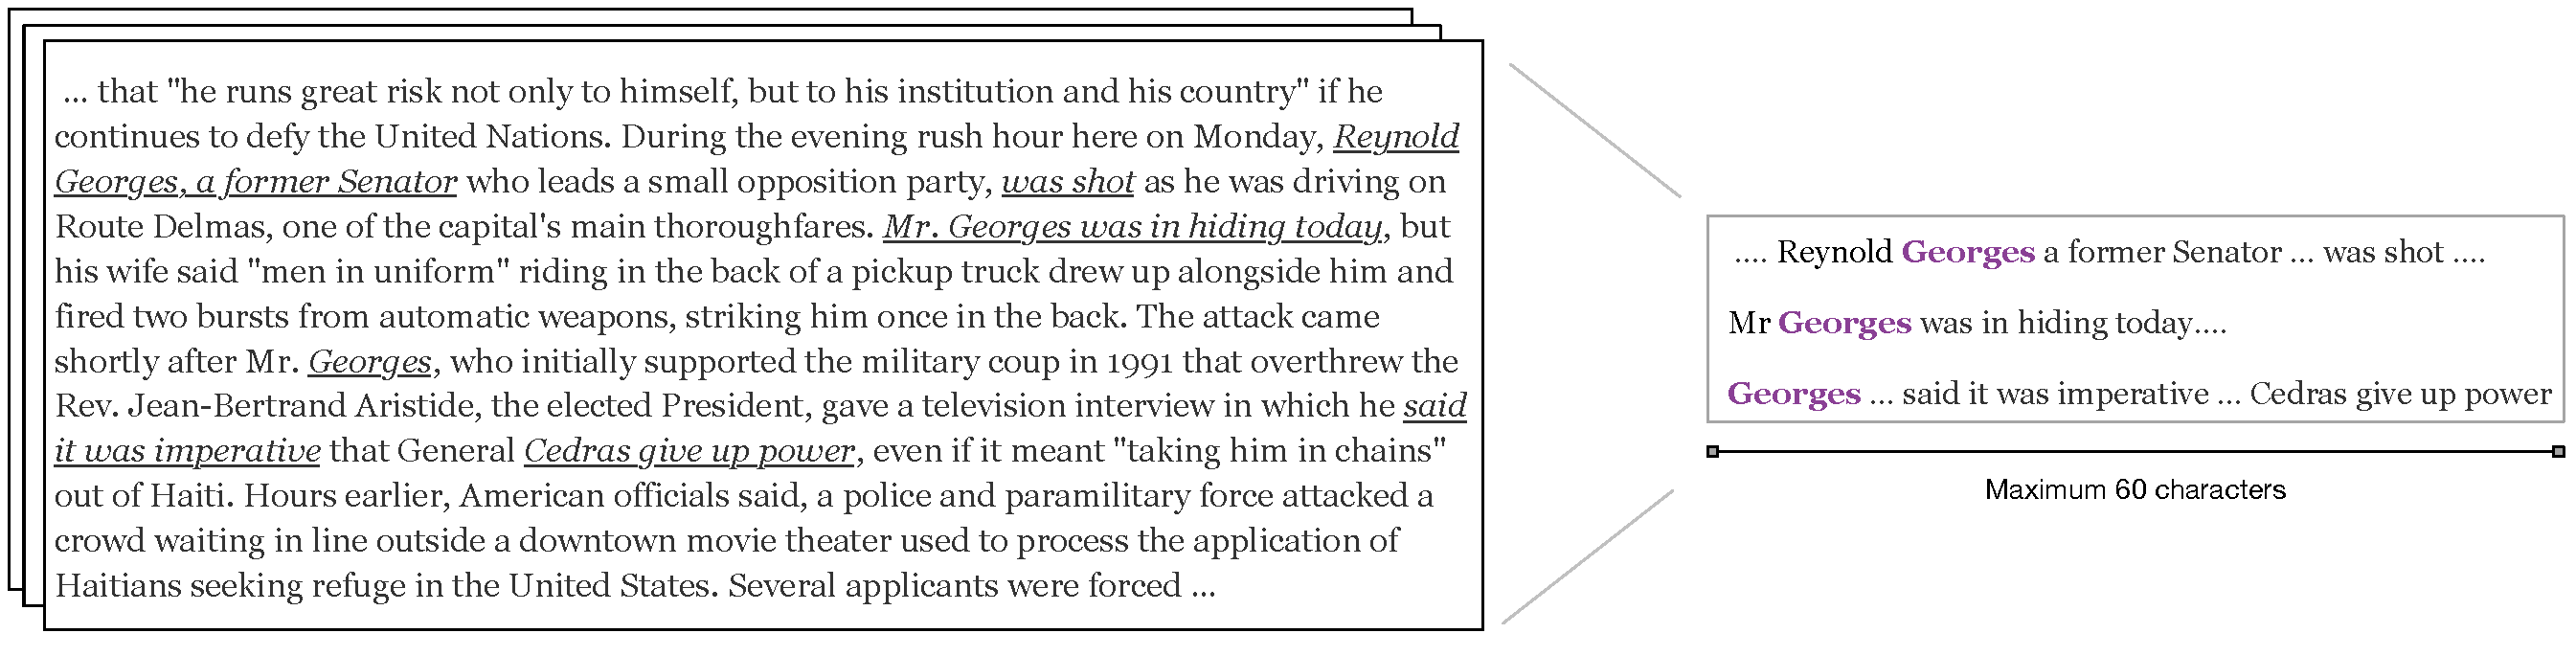
\includegraphics[width=.8\textwidth]{figures/Compression.pdf}
\caption[Text simplification in \ours's Document Feed]{\ours's Document Feed uses text simplification methods from natural language processing in conjunction with color-coded, automatic, in-text highlighting, in order to summarize query mentions \mentions~in context, in a visually consistent format designed for skimming. 
Here one portion of one document (top of stack, left) containing three mentions of the query term $Q$=``Georges'' has been shortened into a summary of ``Georges'' (right). 
To create this summary, \ours~extracts each of the three sentences mentioning ``Georges'' and simplifies each sentence to render a shorter sentence \simplifiedsentence~that is fewer than 60 characters long. 
In this figure, for illustration, spans of tokens from one source document included in the summary are shown with italicized and underlined text. 
In typical use of \ours~there are often hundreds or thousands of documents containing $Q$ (shown as document stack, above left).}\label{f:compressioncartoon}
\end{figure}

{
%%%Replication: $ python token_counter.py

\begin{table}[t!]
\centering
\begin{tabular}{@{}l r@{}}
\toprule
Context       & {Num.\ tokens} \\ \hline 
$\mathcal{C}_{\text{full doc.}} $      & 222,544   \\ 
$\mathcal{C}_{\text{full sent.}}$   & 49,382      \\
$\mathcal{C}_{s^\prime}$  & 28,859    \\  \bottomrule
\end{tabular}
\caption[A quantitative view of how \ours~eases reading burden]{
Total tokens presented to a historian, if each mention of the query ``Reagan'' and subquery ``Duarte'' is shown within the context of a full document ($\mathcal{C}_{\text{full doc.}}$), a full sentence  ($\mathcal{C}_{\text{full sent.}}$) or a shortened sentence ($\mathcal{C}_{s^\prime}$).
By showing shortened sentences, \ours~removes 87.0\% of tokens from all documents containing a query mention, and 41.6\% of tokens from all sentences containing a query mention.
In some cases, removing such tokens will exclude potentially relevant information from the summary; 
in these circumstances, a person would have to find and review such information using the Document Viewer.
Counts come from the example in Figure  \ref{f:system_cc}, using the Salvador corpus (Appendix) and assuming \ours~is shown on a 13-inch screen.
}\label{t:tokens}
\end{table}
}




%. But some sentence

\ours's Document Feed is designed to directly address two of the limitations of baseline \Baselongname~systems, described in Section \ref{s:intro}.
First, by summarizing documents mentioning $Q$, \ours~is able to fit more query mentions in limited screen space, reducing the need for context switching across individual windows or tabs.
For instance, in Figure \ref{f:system_cc}, the Document Feed saves the user from having to open 239 separate documents during comprehensive review.
Second, by selecting sentences mentioning the query from documents, and removing tokens from those sentences, \ours~reduces the user's reading burden.
For instance, in Figure \ref{f:system_cc}, the user has queried for documents mentioning Reagan and Duarte (in this example, Reagan is a subquery; subqueries are described in detail in Section \ref{s:dont_rank_filter}).
By selecting and simplifying sentences, \ours~removes 87.0\% of the tokens in all documents mentioning these two words (Table \ref{t:tokens}).
We include a detailed description of \ours's text simplification techniques in Section \ref{s:simplification}.


\subsection{A linked Document Viewer for necessary context (\rcontext, \rnoconfound)}\label{s:documentviewer}

Because historians need to evaluate evidence in context without black-box algorithmic influence (\rcontext, \rnoconfound), we anticipated that \ours~users would need to quickly review each \specificmention~from the Document Feed within the context of full underlying news articles.
Therefore \ours's Document Feed is closely linked with a corresponding \textbf{Document Viewer}, which shows the complete text of a single selected document from the corpus (Figure \ref{f:system_cc}I).
The Document Viewer satisfies \rcontext~because it shows each \specificmention~within the context of a full document, denoted $\mathcal{C}_{\text{full doc.}}(i)$.
After a user clicks a shortened sentence \simplifiedsentence~in the Document Feed, the Document Viewer updates to show the entire document containing \simplifiedsentence. 
\ours~also automatically scrolls the document so that the (just clicked) simplified sentence is visible on screen.

\ours~also makes it easy for users to locate simplified sentences, by using {automatic in-text highlighting to further link the Document Feed and Document Viewer}.
Each simplified sentence \simplifiedsentence~from the Document Feed is shown with yellow background highlighting 
\includegraphics[scale=0.06]{figures/CCHighlight.pdf} in the document shown in the Document Viewer.
Additionally, if a user hovers over a sentence in the Document Feed or Document Viewer, the sentence is highlighted in dark yellow hover color 
\includegraphics[scale=0.06]{figures/CCHover.pdf} in each component (shown in Figure \ref{f:system_cc}J and \ref{f:system_cc}K).
We hypothesize that linking between shortened text and full documents helps build user trust (\rnoconfound) because it helps experts transparently see and understand how shortened mentions are drawn from underlying text.
This feature is inspired by CommunityClick \cite{CommunityClick}.

\subsection{Color-coded history tracking for systematic review of evidence (\rcomprehensive)}\label{s:tracking}
Some historical researchers emphasize the importance of comprehensively examining all available evidence during research (\rcomprehensive).
To support historians in this work, \ours~keeps track of which documents the analyst clicks in the Document Feed and opens in the Document Viewer.
\ours~also keeps track of bookmarked news stories (Figure \ref{f:system_cc}J), and displays a simple stacked horizontal bar chart (Figure \ref{f:system_cc}G) showing the proportions and counts of read, unread and bookmarked documents. 
The bar chart uses the read 
\includegraphics[scale=0.06]{figures/CCSilver.pdf}, unread 
\includegraphics[scale=0.06]{figures/CCBlack.pdf}, and bookmarked 
\includegraphics[scale=0.06]{figures/CCRed.pdf} color scheme employed across the color-coordinated interface.
(\ours~considers all documents to be either read but not bookmarked, unread or bookmarked. We do not allow intersection between these sets.)
For instance, Figure \ref{f:system_cc}G shows 5 read, 89 unread, and 5 bookmarked documents.
The user can click check marks (Figure \ref{f:system_cc}G) to show or hide documents in each category.

\ours's Document Feed and Time Series View use the same color scheme to help users quickly identify opened and unopened documents. Stories that a user has already clicked appear with grey read text in the Document Feed, and their corresponding rug points are shown in grey in the Time Series View.
For instance, in Figure \ref{f:system_cc}, the user has read the story published on Jan. 9, 1985.
The story is greyed out in the Document Feed, and its corresponding rug point is shown in grey beneath the time series plot.
Similarly, there are five red rug points in Figure \ref{f:system_cc}E because the user has bookmarked five documents.

Note that \ours's history tracking is query-dependent; tracking resets each time a user issues a new query (unlike the history tracking mechanism in some prior work \cite[Section 6]{Footprints}).
Such query-dependent tracking is appropriate for \ours~because the system is designed to help historians review all mentions of some specific keyword in a corpus.
We hypothesize that this feature offers experts assurance they have comprehensively reviewed all \specificmention. 
We leave exploration of other forms of history tracking for future work.

\subsection{A filtering system to review many results in a neutral manner (\rnoconfound)}\label{s:dont_rank_filter}

Some prior text analysis systems designed for historians (e.g., Expedition \cite{expedition}) attempt to answer keyword queries by ranking documents to direct users towards most-relevant news articles.
Because such ranked retrieval might introduce unwanted algorithmic influence over the expert search process (\rnoconfound), \ours~responds to queries with Boolean search, which returns the unranked set of all documents containing $Q$.
(The Document Feed shows such documents in chronological order.)
\ours~then allows users to narrow down unranked search results with a filtering system, consisting of three filter controls.

The \textbf{filter-by-date} control selects documents by time period. After users select a start date and end date from date pickers at the top of the interface (Figure \ref{f:system_cc}B), \ours~updates to show only those documents mentioning the query published during the selected interval.
(Historians are often interested in specific time periods; see Section \ref{s:needs}.)
In Figure \ref{f:system_cc}B, the user has filtered to documents published in 1983--1985.

The \textbf{filter-by-subquery} control allows users to select documents that contain some additional word, called a subquery. For instance, after a user queries for the Salvadoran leader ``{Duarte}'' they might wish to further narrow results to understand the relationship between ``{Duarte}'' and his ally U.S.\ President Ronald Reagan.
To investigate, the user can enter the subquery ``{Reagan}'' to select all documents mentioning the word ``{Duarte}'' which also mention the query word ``{Reagan}'' (Figure \ref{f:system_cc}C).
We included this feature because complex Boolean queries are often popular with experts \cite[Section 1.4]{irbook}.
More complex Boolean expressions are possible in future work.

The \textbf{filter-by-count} control filters results based on the the number of times a query term is mentioned in a document.
When a user adjusts the filter-by-count slider to some value $K \in \{1,2,3,4,5\}$ all components of the interface update to show only those documents with $K$ or more \specificmention.
In cases where a user has set a subquery, the filter-by-count control allows the user to select documents which contain the subquery word at least $K$ times.
For instance, in Figure \ref{f:system_cc}F, the user selects documents which mention ``{Reagan}'' at least 3 times.

\ours~also helps users quickly see the count of query terms within documents using square-shaped, query-colored \textbf{count markers}, shown beside each document headline.
Count markers use brightness to encode the count of a query term within a document.
For instance, count markers for documents with more mentions of a query term have a darker purple color than count markers for documents with fewer mentions.
If a user enters a subquery, count markers show the count of the subquery within each document, using shades of the subquery color (as in Figure \ref{f:system_cc}F and \ref{f:system_cc}H).
This feature is inspired by TileBars \cite{TileBars}.

\subsection{Sentence simplification to help summarize a query across a corpus}\label{s:simplification}

\ours~introduces text simplification methods from NLP to the literature on text analytics. We describe these methods below.

\subsubsection{Overview of sentence simplification in \ours}\label{s:text_simplification_overview}

\ours's Document Feed displays a query-focused summary of a user's query and subquery, by first extracting and then simplifying sentences mentioning query (or subquery) words.
To simplify sentences, we turn to sentence compression techniques from the text summarization literature in NLP (introduced in Section \ref{s:textual_summary_family}).
These methods try to summarize naturally-occurring input sentences by removing words, to create shorter and well-formed output sentences which contain the most salient information from the input.
(A well-formed sentence is one that sounds natural, rather than garbled or choppy \cite{sprouseschutzeintro}.)
In particular, we turn to a specific class of sentence compression methods, which can ensure that simplified sentences both (A) fit within limited screen space in a user interface and (B) mention the user's query term or subquery term. 
Such methods are appropriate for \ours~because each line in the Document Feed has a fixed width, and must include some mention of the user's query or subquery.

More concretely, we use a \textit{query-focused clause deletion} \cite{Handler2019HumanAJ,Handler2019Query} method to shorten sentences in cases when a user has entered a query (Section \ref{s:clause_deletion}),
and also use \textit{relationship span extraction} method \cite{handler-oconnor-2018-relational} in cases when a user has entered both a query and subquery (Section \ref{s:rsum_extraction}).
We also employ a final fallback approach, \textit{character windowing},
when it is not possible to shorten a sentence using other techniques (Section \ref{s:clause_deletion}).
In the next sections, we describe each sentence shortening method in greater detail. The Appendix provides additional details on how \ours~chooses between possible sentence shortening methods.\footnote{
In Figure \ref{f:system_cc}, \ours~uses relationship span extraction to shorten and display some sentence from 31 out of 239 documents which mention ``Duarte'' and ``Reagan.'' 
It uses query-focused clause deletion to shorten and display some sentence from 85 documents, and it resorts to character windowing for the remaining 123 documents.\label{footnote_counts}}

\subsubsection{Query-focused clause deletion, and character windowing}\label{s:clause_deletion}

\ours's Document Feed requires shortened sentences that mention $Q$ and fit within available screen space.
We assume that such shortenings should also be well-formed and contain the most salient information from longer source sentences. 
Prior research in IR suggests that users prefer well-formed snippets \cite{ryenwhitesnippets}, and prior work in sentence compression \cite{Knight2000StatisticsBasedS,filippova-altun-2013-overcoming, filippova2015sentence} strives for both well-formedness and salience.
We also assume that methods for constructing shortenings must run with low latency, which is known to be important in user-facing analytics systems \cite{latencyliu}.
Different sentence shortening techniques might optimize for and manage tradeoffs between such requirements. 
But in this work we turn to a simple \textit{query-focused clause deletion} method to meet such criteria, allowing us to focus on how to apply text summarization methods in user interfaces for historical research.

Query-focused clause deletion exploits the fact that natural language sentences are sequences of words, which exhibit hierarchical and nested grammatical structure \cite{bender_linguistic_2013}.
For instance, the sequence ``She swims in the pool'' can be divided into interrelated word groups, with specific grammatical relationships; the words ``in the pool'' form a prepositional phrase that modifies the verb ``swims.''
To represent such linguistic structure, clause deletion employs a dependency parse tree \cite{Nivre2016UniversalDV} grammatical formalism.
A dependency parse is a directed tree graph with one vertex for each word in the sentence, along with a latent root vertex.\footnote{We use the UD (v1) dependency formalism \cite{Nivre2016UniversalDV}; other related formalisms allow for non-tree parses \cite{schuster-manning-2016-enhanced}. Eisenstein \cite[Chapter 11]{eisenstein2019introduction} offers a broad introduction to dependencies. We perform dependency parsing using Stanford CoreNLP \cite{corenlppipeline,chen-manning-2014-fast}.}
Each subtree in the parse corresponds to a constituent subsequence in the sentence. 
The sentence simplification literature sometimes describes such subtrees as \textit{clauses} \cite{filippova-strube-2008-dependency}.
Figure \ref{f:clause_deletion_1} shows an example dependency parse.

Sentence simplification via {clause deletion} shortens sentences by iteratively deleting clauses from a dependency parse.\footnote{Tokens from the remaining tree are then printed in left-to-right order, based on their position in the original sentence.}
Figure \ref{f:clause_deletion} shows how one sentence is shortened by iteratively deleting two clauses.
Unlike sentence compression techniques which consider individual tokens for removal (e.g., Filippova et al.\ \cite{filippova2015sentence}), deleting clauses naturally identifies and removes groups of related words.
For example, a single deletion could remove the prepositional phrase ``after the election,'' or a much longer word group with more modifiers and embedded clauses: ``after the previous election last year, which went poorly.''
Shortening sentences via clause deletion also makes it easy to ensure that output sentences must include $Q$; clauses that contain query mentions are not allowed to be removed during deletion.\footnote{
It is also possible to enforce such query constraints using integer linear programming (ILP). 
However, ILP-based sentence compression techniques (e.g., Clarke and Lapata \ \cite{clarke2008}) are NP-hard and have been shown to be orders of magnitude slower than other iterative approaches to query-focused sentence compression \cite{Handler2019Query}.
}



\begin{figure}
  \begin{subfigure}[t]{\textwidth}
    \centering
    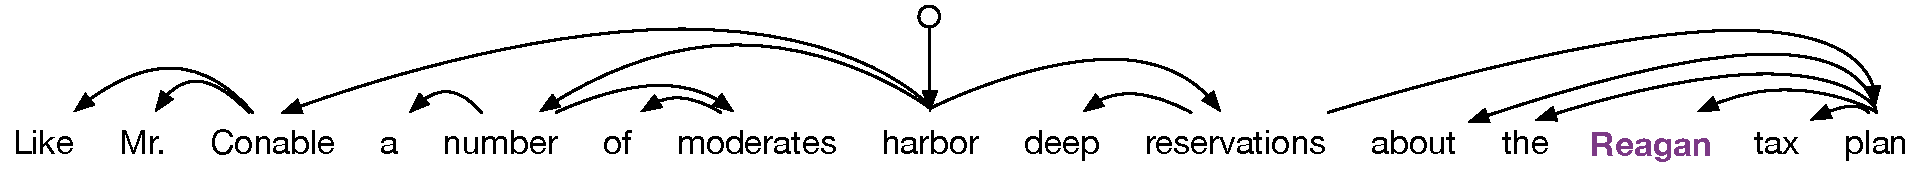
\includegraphics[width=.65\textwidth]{figures/clause_deletion/clause_deletion_one.pdf}
    \caption[]{An untyped dependency parse tree %\cite{Nivre2016UniversalDV} 
    of an input sentence mentioning $Q$=``Reagan.''}\label{f:clause_deletion_1}
  \end{subfigure}\hfill
  \begin{subfigure}[t]{\textwidth}
    \centering
    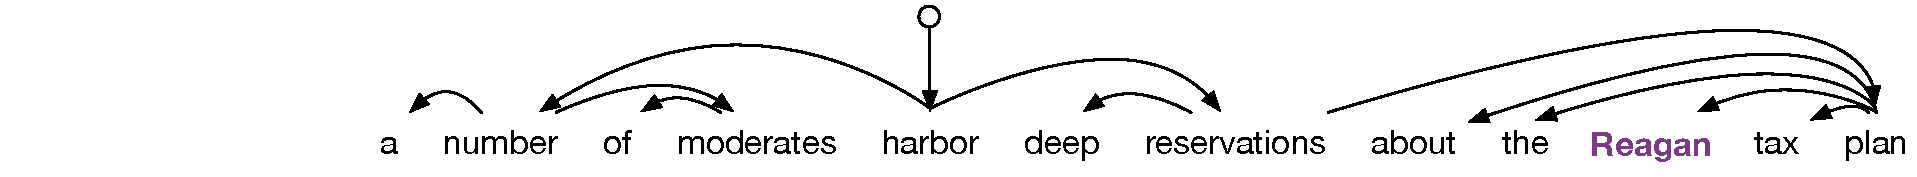
\includegraphics[width=.65\textwidth]{figures/clause_deletion/clause_deletion_two.pdf}
    \caption[]{To simplify the sentence, \ours~ first removes the clause (subtree) ``Like Mr. Conable.''}\label{f:clause_deletion_2}
  \end{subfigure}
   \begin{subfigure}[t]{\textwidth}
    \centering
    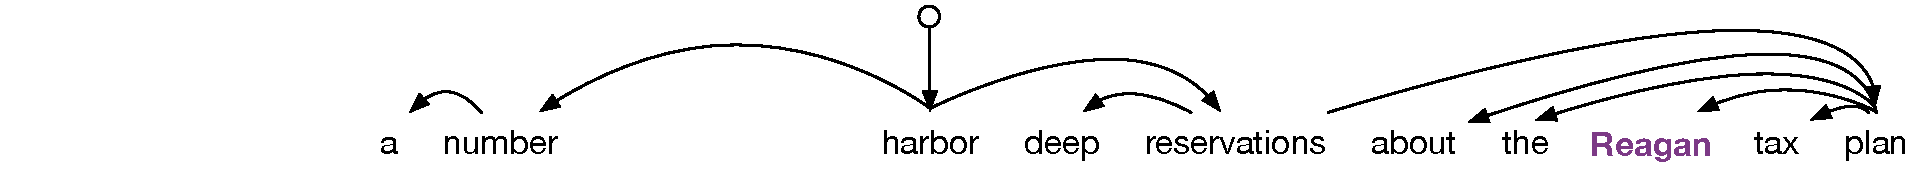
\includegraphics[width=.65\textwidth]{figures/clause_deletion/clause_deletion_three.pdf}
    \caption[]{In this step, \ours~removes another clause that does not contain $Q$.\vspace{.25 cm}}\label{f:clause_deletion_3}
  \end{subfigure}
  \caption[Sentence simplification via query-focused clause deletion]{Sentence simplification via query-focused clause deletion \cite{Handler2019Query,Handler2019HumanAJ}. \ours~removes two subtrees from a dependency parse across two steps to simplify the input sentence (\ref{f:clause_deletion_1}) into the output sentence (\ref{f:clause_deletion_3}).}\label{f:clause_deletion}
\end{figure}


To try and create well-formed output sentences, \ours~turns to prior work on clause deletion \cite[Section 6]{Handler2019HumanAJ}, which has found that in general removing more clauses from an input sentence makes it less likely that the resulting output sentence will be well-formed.
Thus, to shorten an input sentence, \ours's clause deletion first identifies those candidate output shortenings that can be constructed by removing at most $K$ clauses from the input (without removing $Q$), and are also short enough to fit in one line of text within the Document Feed.
Because in practice it is often possible to dramatically shorten an English news sentence by removing only one or two large clauses (for example, a lengthy relative clause, such as ``Reagan met with the envoy \sout{who was sent by the ...}''), \ours~only considers shortenings which can be constructed by removing 
$0 < K \leq 2$ deletions.\footnote{
In addition to encouraging well-formed output, this strict limit ensures low latency for the user.
For a sentence $M$ words long, the worst case for performance is a tree where all words are leaf vertexes, resulting in $M+M(M-1)/2$ possible outputs of $K=1$ or $2$ deletions.
But in typical trees, there are far fewer possible deletions because: (1) the query word and all its ancestors are not allowed to be deleted, (2) after the first deletion of a clause length $C$ (i.e., the size of the deleted subtree) only $M-C$ candidates remain for the second deletion, and (3) if \ours~finds any candidate shortenings using $K$=1, it won't search for candidates using $K$=2, as shortenings which remove fewer clauses are more likely to be well-formed.
We do not consider cases where $K=0$, as most unshortened news sentences are too long to fit within the Document Viewer.}

To try and ensure that output shortenings include the most salient information from input sentences, \ours~then returns the candidate output shortening with the highest tf-idf score \cite{irbook}.
Tf-idf scores are often used in extractive sentence compression
\cite{clarke2008,filippova-strube-2008-dependency} and text summarization \cite{das2007survey} to identify salient information for inclusion in summary output;
this metric identifies words which occur with unusual frequency (relative to the overall corpus), which is an important signal of salience in summarization \cite{sumbasic}.
The Appendix includes details of how we compute td-idf in \ours~to identify words which occur frequently in documents mentioning a query.


In some cases, there is no way to shorten a sentence by removing one or two clauses while ensuring that that output sentence mentions $Q$ and will fit in the Document Feed. 
In these circumstances, \ours~resorts to shortening the sentence by extracting the span of $N$ characters to the left and right of $Q$ in the sentence, where we maximize $N$ under the constraint that the resulting character span will both fit in Document Feed and respect word boundaries.
We use this \textit{character windowing} method only as a last resort because it may cut off syntactic constituents (e.g., show only a portion of a prepositional phrase), which may create awkward-sounding output.
\Cref{footnote_counts} describes how often \ours~uses this fallback, during an example run of \ours. 

In the future, it might be possible to shorten more sentences with query-focused clause deletion by considering candidate output shortenings that are created using more than $K=2$ deletions.
(Prior work on query-focused clause deletion does not yet offer an efficient solution for considering such candidates \cite{Handler2019HumanAJ}.)
Because the number of candidates grows with $K$, developing algorithms which efficiently search over possible outputs or learn greedy deletion policies based on data (e.g., with reinforcement learning) might offer useful starting points. 


\subsubsection{Relationship span extraction}\label{s:rsum_extraction}

\ours~users who search for a query term $Q$ can also filter query results by a subquery.
When a user enters both a query and a subquery term, we assume that they are broadly interested in how these two terms are related in the corpus.
For instance, a user might query for the Salvadoran leader  $Q$=``Duarte'' and apply a subquery for the then U.S.\ President ``Reagan,'' in order to understand Duarte's relationship to Reagan (Figure \ref{f:system_cc}). 

\begin{figure}[t!]
    \centering
    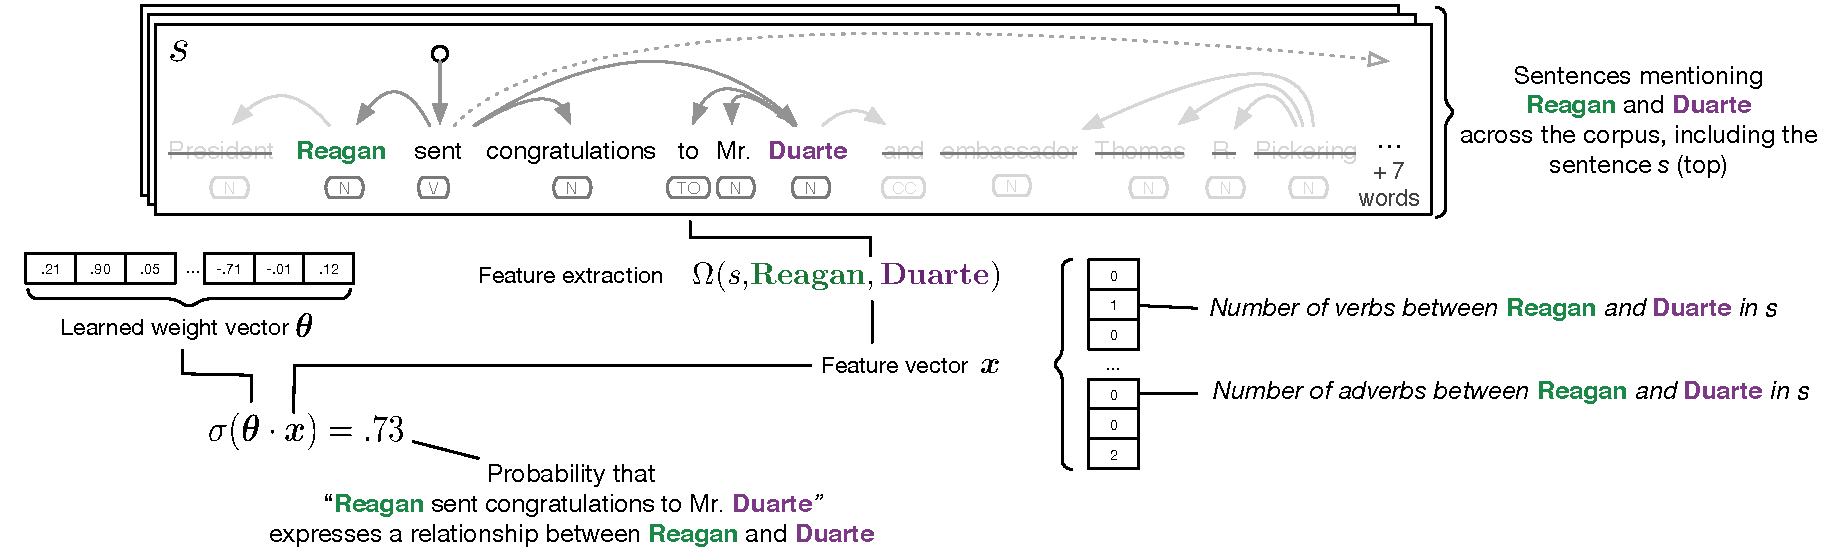
\includegraphics[width=.9\textwidth]{figures/rsum/rsum_big.pdf}
    \caption[Sentence simplification via relationship span extraction]{Sentence simplification via relationship span extraction \cite{handler-oconnor-2018-relational}.
    This method predicts the probability that the span of tokens between the query and subquery words in a given sentence $s$ will sound natural as a shorter and standalone sentence.
    (If the predicted probability is high, the sentence can likely be shortened to the span of tokens.)
    This figure shows the predicted probability that the token span between the query \textbf{\color{CCPurple}{Duarte}} and the subquery \textbf{\color{darkgreen}{Reagan}} will sound natural as a shortened sentence when extracted from the longer sentence shown in Figure \ref{f:system_cc} (letter K).
    Seven words from $s$ are not shown in the diagram above.}\label{f:rsum}
\end{figure}


% {\color[rgb]{0.000000,0.000000,0.000000}\Omega(s,} {\color[rgb]{.106, .471, .216}\text{\textbf{Reagan}}}, {\color[rgb]{.405, .144, .450}\text{\textbf{Duarte}}}{\color[rgb]{0.000000,0.000000,0.000000})}=\boldsymbol{x}_i 

To meet this information need, \ours~attempts to simplify long and complex sentences mentioning both the query and subquery terms into short sentences which concisely describe the {relationship} between the query and subquery.
We describe the process of shortening sentences in this manner as \textit{relationship span extraction} because each shortened sentence is a token span (i.e., sequence of tokens) extracted from a longer sentence. 
For instance, in Figure \ref{f:system_cc}, we extract the span ``Reagan sent congratulations to Mr.\ Duarte'' from the longer sentence ``{\color{gray}\sout{President}} Reagan sent congratulations to Mr. Duarte {\color{gray}\sout{and Ambassador Thomas R. Pickering pledged United States support for further meetings}}.''

\ours~relies on a known natural language processing technique to perform relationship span extraction, which is specified in detail in prior literature \cite[Sec.\ 4]{handler-oconnor-2018-relational}.
At a high-level, this method employs logistic regression to determine if an input sentence $s$ containing two input query words can be shortened to express a relationship between those two query words. 
To make this determination, the method first extracts a vector of linguistic features $\bm{x}$ containing information about the query words in the sentence  (e.g., is there a verb token between the query words in $s$?), and then passes the dot product of $\bm{x}$ and a learned weight vector $\bm{\theta}$ through a logistic function $\sigma$. This returns a predicted probability that the token span between the query and subquery will sound natural when removed from the sentence (Figure \ref{f:rsum}).
In our case, the input query words are the user's query and subquery;
we shorten a sentence $s$ to a relationship span if the predicted probability that the span sounds natural is greater than a threshold $T=0.5$.\footnote{We implement with Scikit-learn \cite{Pedregosa:2011:SML:1953048.2078195}. Note that setting a lower threshold $T$ might increase the total number of shortened sentences, at the cost of creating fewer well-formed extractions (and vice versa).}

In our implementation of \ours (as in prior literature \cite{handler-oconnor-2018-relational}), relationship span extraction is supervised using a benchmark corpus from \citet{filippova-altun-2013-overcoming}, consisting of single sentences paired with single-sentence summaries, which are automatically generated from news headlines.
In principle, a technically-oriented \ours~user would be able to retrain relationship span extraction on their own corpus, using the technique from Filippova and Altun to automatically generate training data from headlines in their own news archive.
